\documentclass[1p]{elsarticle_modified}
%\bibliographystyle{elsarticle-num}

%\usepackage[colorlinks]{hyperref}
%\usepackage{abbrmath_seonhwa} %\Abb, \Ascr, \Acal ,\Abf, \Afrak
\usepackage{amsfonts}
\usepackage{amssymb}
\usepackage{amsmath}
\usepackage{amsthm}
\usepackage{scalefnt}
\usepackage{amsbsy}
\usepackage{kotex}
\usepackage{caption}
\usepackage{subfig}
\usepackage{color}
\usepackage{graphicx}
\usepackage{xcolor} %% white, black, red, green, blue, cyan, magenta, yellow
\usepackage{float}
\usepackage{setspace}
\usepackage{hyperref}

\usepackage{tikz}
\usetikzlibrary{arrows}

\usepackage{multirow}
\usepackage{array} % fixed length table
\usepackage{hhline}

%%%%%%%%%%%%%%%%%%%%%
\makeatletter
\renewcommand*\env@matrix[1][\arraystretch]{%
	\edef\arraystretch{#1}%
	\hskip -\arraycolsep
	\let\@ifnextchar\new@ifnextchar
	\array{*\c@MaxMatrixCols c}}
\makeatother %https://tex.stackexchange.com/questions/14071/how-can-i-increase-the-line-spacing-in-a-matrix
%%%%%%%%%%%%%%%

\usepackage[normalem]{ulem}

\newcommand{\msout}[1]{\ifmmode\text{\sout{\ensuremath{#1}}}\else\sout{#1}\fi}
%SOURCE: \msout is \stkout macro in https://tex.stackexchange.com/questions/20609/strikeout-in-math-mode

\newcommand{\cancel}[1]{
	\ifmmode
	{\color{red}\msout{#1}}
	\else
	{\color{red}\sout{#1}}
	\fi
}

\newcommand{\add}[1]{
	{\color{blue}\uwave{#1}}
}

\newcommand{\replace}[2]{
	\ifmmode
	{\color{red}\msout{#1}}{\color{blue}\uwave{#2}}
	\else
	{\color{red}\sout{#1}}{\color{blue}\uwave{#2}}
	\fi
}

\newcommand{\Sol}{\mathcal{S}} %segment
\newcommand{\D}{D} %diagram
\newcommand{\A}{\mathcal{A}} %arc


%%%%%%%%%%%%%%%%%%%%%%%%%%%%%5 test

\def\sl{\operatorname{\textup{SL}}(2,\Cbb)}
\def\psl{\operatorname{\textup{PSL}}(2,\Cbb)}
\def\quan{\mkern 1mu \triangleright \mkern 1mu}

\theoremstyle{definition}
\newtheorem{thm}{Theorem}[section]
\newtheorem{prop}[thm]{Proposition}
\newtheorem{lem}[thm]{Lemma}
\newtheorem{ques}[thm]{Question}
\newtheorem{cor}[thm]{Corollary}
\newtheorem{defn}[thm]{Definition}
\newtheorem{exam}[thm]{Example}
\newtheorem{rmk}[thm]{Remark}
\newtheorem{alg}[thm]{Algorithm}

\newcommand{\I}{\sqrt{-1}}
\begin{document}

%\begin{frontmatter}
%
%\title{Boundary parabolic representations of knots up to 8 crossings}
%
%%% Group authors per affiliation:
%\author{Yunhi Cho} 
%\address{Department of Mathematics, University of Seoul, Seoul, Korea}
%\ead{yhcho@uos.ac.kr}
%
%
%\author{Seonhwa Kim} %\fnref{s_kim}}
%\address{Center for Geometry and Physics, Institute for Basic Science, Pohang, 37673, Korea}
%\ead{ryeona17@ibs.re.kr}
%
%\author{Hyuk Kim}
%\address{Department of Mathematical Sciences, Seoul National University, Seoul 08826, Korea}
%\ead{hyukkim@snu.ac.kr}
%
%\author{Seokbeom Yoon}
%\address{Department of Mathematical Sciences, Seoul National University, Seoul, 08826,  Korea}
%\ead{sbyoon15@snu.ac.kr}
%
%\begin{abstract}
%We find all boundary parabolic representation of knots up to 8 crossings.
%
%\end{abstract}
%\begin{keyword}
%    \MSC[2010] 57M25 
%\end{keyword}
%
%\end{frontmatter}

%\linenumbers
%\tableofcontents
%
\newcommand\colored[1]{\textcolor{white}{\rule[-0.35ex]{0.8em}{1.4ex}}\kern-0.8em\color{red} #1}%
%\newcommand\colored[1]{\textcolor{white}{ #1}\kern-2.17ex	\textcolor{white}{ #1}\kern-1.81ex	\textcolor{white}{ #1}\kern-2.15ex\color{red}#1	}

{\Large $\underline{11a_{8}~(K11a_{8})}$}

\setlength{\tabcolsep}{10pt}
\renewcommand{\arraystretch}{1.6}
\vspace{1cm}\begin{tabular}{m{100pt}>{\centering\arraybackslash}m{274pt}}
\multirow{5}{120pt}{
	\centering
	\includegraphics[width=112pt]{../../../GIT/diagram.site/Diagrams/png/257_11a_8.png}\\
\ \ \ A knot diagram\footnotemark}&
\allowdisplaybreaks
\textbf{Linearized knot diagam} \\
\cline{2-2}
 &
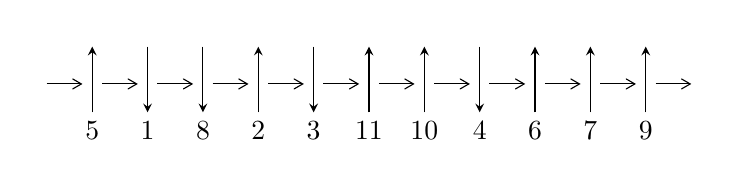
\begin{tikzpicture}[x=20pt, y=17pt]
	% nodes
	\node (C0) at (0, 0) {};
	\node (C1) at (1, 0) {};
	\node (C1U) at (1, +1) {};
	\node (C1D) at (1, -1) {5};

	\node (C2) at (2, 0) {};
	\node (C2U) at (2, +1) {};
	\node (C2D) at (2, -1) {1};

	\node (C3) at (3, 0) {};
	\node (C3U) at (3, +1) {};
	\node (C3D) at (3, -1) {8};

	\node (C4) at (4, 0) {};
	\node (C4U) at (4, +1) {};
	\node (C4D) at (4, -1) {2};

	\node (C5) at (5, 0) {};
	\node (C5U) at (5, +1) {};
	\node (C5D) at (5, -1) {3};

	\node (C6) at (6, 0) {};
	\node (C6U) at (6, +1) {};
	\node (C6D) at (6, -1) {11};

	\node (C7) at (7, 0) {};
	\node (C7U) at (7, +1) {};
	\node (C7D) at (7, -1) {10};

	\node (C8) at (8, 0) {};
	\node (C8U) at (8, +1) {};
	\node (C8D) at (8, -1) {4};

	\node (C9) at (9, 0) {};
	\node (C9U) at (9, +1) {};
	\node (C9D) at (9, -1) {6};

	\node (C10) at (10, 0) {};
	\node (C10U) at (10, +1) {};
	\node (C10D) at (10, -1) {7};

	\node (C11) at (11, 0) {};
	\node (C11U) at (11, +1) {};
	\node (C11D) at (11, -1) {9};
	\node (C12) at (12, 0) {};

	% arrows
	\draw[->,>={angle 60}]
	(C0) edge (C1) (C1) edge (C2) (C2) edge (C3) (C3) edge (C4) (C4) edge (C5) (C5) edge (C6) (C6) edge (C7) (C7) edge (C8) (C8) edge (C9) (C9) edge (C10) (C10) edge (C11) (C11) edge (C12) ;	\draw[->,>=stealth]
	(C1D) edge (C1U) (C2U) edge (C2D) (C3U) edge (C3D) (C4D) edge (C4U) (C5U) edge (C5D) (C6D) edge (C6U) (C7D) edge (C7U) (C8U) edge (C8D) (C9D) edge (C9U) (C10D) edge (C10U) (C11D) edge (C11U) ;
	\end{tikzpicture} \\
\hhline{~~} \\& 
\textbf{Solving Sequence} \\ \cline{2-2} 
 &
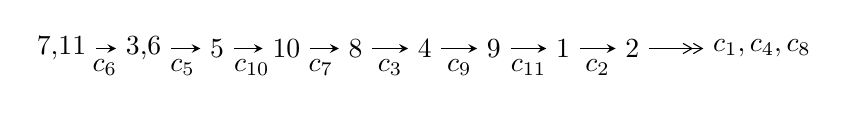
\begin{tikzpicture}[x=25pt, y=7pt]
	% node
	\node (A0) at (-1/8, 0) {7,11};
	\node (A1) at (17/16, 0) {3,6};
	\node (A2) at (17/8, 0) {5};
	\node (A3) at (25/8, 0) {10};
	\node (A4) at (33/8, 0) {8};
	\node (A5) at (41/8, 0) {4};
	\node (A6) at (49/8, 0) {9};
	\node (A7) at (57/8, 0) {1};
	\node (A8) at (65/8, 0) {2};
	\node (C1) at (1/2, -1) {$c_{6}$};
	\node (C2) at (13/8, -1) {$c_{5}$};
	\node (C3) at (21/8, -1) {$c_{10}$};
	\node (C4) at (29/8, -1) {$c_{7}$};
	\node (C5) at (37/8, -1) {$c_{3}$};
	\node (C6) at (45/8, -1) {$c_{9}$};
	\node (C7) at (53/8, -1) {$c_{11}$};
	\node (C8) at (61/8, -1) {$c_{2}$};
	\node (A9) at (10, 0) {$c_{1},c_{4},c_{8}$};

	% edge
	\draw[->,>=stealth]	
	(A0) edge (A1) (A1) edge (A2) (A2) edge (A3) (A3) edge (A4) (A4) edge (A5) (A5) edge (A6) (A6) edge (A7) (A7) edge (A8) ;
	\draw[->>,>={angle 60}]	
	(A8) edge (A9);
\end{tikzpicture} \\ 

\end{tabular} \\

\footnotetext{
The image of knot diagram is generated by the software ``\textbf{Draw programme}" developed by Andrew Bartholomew(\url{http://www.layer8.co.uk/maths/draw/index.htm\#Running-draw}), where we modified some parts for our purpose(\url{https://github.com/CATsTAILs/LinksPainter}).
}\phantom \\ \newline 
\centering \textbf{Ideals for irreducible components\footnotemark of $X_{\text{par}}$} 
 
\begin{align*}
I^u_{1}&=\langle 
4 u^{63}-11 u^{62}+\cdots+2 b-2,\;-5 u^{63}+14 u^{62}+\cdots+2 a+12,\;u^{64}-3 u^{63}+\cdots-3 u+1\rangle \\
I^u_{2}&=\langle 
- u^2 a- a u+b,\;- u^2 a+a^2- a u+2 u^2-2 a+u+3,\;u^3+u^2+2 u+1\rangle \\
\\
\end{align*}
\raggedright * 2 irreducible components of $\dim_{\mathbb{C}}=0$, with total 70 representations.\\
\footnotetext{All coefficients of polynomials are rational numbers. But the coefficients are sometimes approximated in decimal forms when there is not enough margin.}
\newpage
\renewcommand{\arraystretch}{1}
\centering \section*{I. $I^u_{1}= \langle 4 u^{63}-11 u^{62}+\cdots+2 b-2,\;-5 u^{63}+14 u^{62}+\cdots+2 a+12,\;u^{64}-3 u^{63}+\cdots-3 u+1 \rangle$}
\flushleft \textbf{(i) Arc colorings}\\
\begin{tabular}{m{7pt} m{180pt} m{7pt} m{180pt} }
\flushright $a_{7}=$&$\begin{pmatrix}1\\0\end{pmatrix}$ \\
\flushright $a_{11}=$&$\begin{pmatrix}0\\u\end{pmatrix}$ \\
\flushright $a_{3}=$&$\begin{pmatrix}\frac{5}{2} u^{63}-7 u^{62}+\cdots+7 u-6\\-2 u^{63}+\frac{11}{2} u^{62}+\cdots-\frac{1}{2} u+1\end{pmatrix}$ \\
\flushright $a_{6}=$&$\begin{pmatrix}1\\u^2\end{pmatrix}$ \\
\flushright $a_{5}=$&$\begin{pmatrix}\frac{1}{2} u^{63}- u^{62}+\cdots+4 u+1\\-\frac{1}{2} u^{62}+u^{61}+\cdots-\frac{5}{2} u^2-\frac{1}{2} u\end{pmatrix}$ \\
\flushright $a_{10}=$&$\begin{pmatrix}- u\\u\end{pmatrix}$ \\
\flushright $a_{8}=$&$\begin{pmatrix}u^2+1\\- u^2\end{pmatrix}$ \\
\flushright $a_{4}=$&$\begin{pmatrix}\frac{9}{2} u^{63}-10 u^{62}+\cdots+8 u-7\\-4 u^{63}+\frac{17}{2} u^{62}+\cdots-\frac{1}{2} u+1\end{pmatrix}$ \\
\flushright $a_{9}=$&$\begin{pmatrix}- u^3-2 u\\- u^5- u^3+u\end{pmatrix}$ \\
\flushright $a_{1}=$&$\begin{pmatrix}u^7+4 u^5+4 u^3\\u^9+3 u^7+u^5-2 u^3+u\end{pmatrix}$ \\
\flushright $a_{2}=$&$\begin{pmatrix}4 u^{63}-9 u^{62}+\cdots+\frac{17}{2} u-\frac{13}{2}\\-3 u^{63}+6 u^{62}+\cdots+\frac{3}{2} u+\frac{1}{2}\end{pmatrix}$\\ \flushright $a_{2}=$&$\begin{pmatrix}4 u^{63}-9 u^{62}+\cdots+\frac{17}{2} u-\frac{13}{2}\\-3 u^{63}+6 u^{62}+\cdots+\frac{3}{2} u+\frac{1}{2}\end{pmatrix}$\\&\end{tabular}
\flushleft \textbf{(ii) Obstruction class $= -1$}\\~\\
\flushleft \textbf{(iii) Cusp Shapes $= u^{63}-\frac{3}{2} u^{62}+\cdots+7 u+\frac{1}{2}$}\\~\\
\newpage\renewcommand{\arraystretch}{1}
\flushleft \textbf{(iv) u-Polynomials at the component}\newline \\
\begin{tabular}{m{50pt}|m{274pt}}
Crossings & \hspace{64pt}u-Polynomials at each crossing \\
\hline $$\begin{aligned}c_{1},c_{4}\end{aligned}$$&$\begin{aligned}
&u^{64}+4 u^{63}+\cdots+4 u+1
\end{aligned}$\\
\hline $$\begin{aligned}c_{2}\end{aligned}$$&$\begin{aligned}
&u^{64}+32 u^{63}+\cdots+4 u+1
\end{aligned}$\\
\hline $$\begin{aligned}c_{3},c_{8}\end{aligned}$$&$\begin{aligned}
&u^{64}- u^{63}+\cdots+32 u+64
\end{aligned}$\\
\hline $$\begin{aligned}c_{5}\end{aligned}$$&$\begin{aligned}
&u^{64}-4 u^{63}+\cdots+393 u+306
\end{aligned}$\\
\hline $$\begin{aligned}c_{6},c_{7},c_{10}\end{aligned}$$&$\begin{aligned}
&u^{64}+3 u^{63}+\cdots+3 u+1
\end{aligned}$\\
\hline $$\begin{aligned}c_{9}\end{aligned}$$&$\begin{aligned}
&u^{64}-3 u^{63}+\cdots+139 u+34
\end{aligned}$\\
\hline $$\begin{aligned}c_{11}\end{aligned}$$&$\begin{aligned}
&u^{64}+13 u^{63}+\cdots+9803 u+563
\end{aligned}$\\
\hline
\end{tabular}\\~\\
\newpage\renewcommand{\arraystretch}{1}
\flushleft \textbf{(v) Riley Polynomials at the component}\newline \\
\begin{tabular}{m{50pt}|m{274pt}}
Crossings & \hspace{64pt}Riley Polynomials at each crossing \\
\hline $$\begin{aligned}c_{1},c_{4}\end{aligned}$$&$\begin{aligned}
&y^{64}+32 y^{63}+\cdots+4 y+1
\end{aligned}$\\
\hline $$\begin{aligned}c_{2}\end{aligned}$$&$\begin{aligned}
&y^{64}+4 y^{63}+\cdots+32 y+1
\end{aligned}$\\
\hline $$\begin{aligned}c_{3},c_{8}\end{aligned}$$&$\begin{aligned}
&y^{64}-35 y^{63}+\cdots-62464 y+4096
\end{aligned}$\\
\hline $$\begin{aligned}c_{5}\end{aligned}$$&$\begin{aligned}
&y^{64}-24 y^{63}+\cdots-628749 y+93636
\end{aligned}$\\
\hline $$\begin{aligned}c_{6},c_{7},c_{10}\end{aligned}$$&$\begin{aligned}
&y^{64}+59 y^{63}+\cdots+9 y+1
\end{aligned}$\\
\hline $$\begin{aligned}c_{9}\end{aligned}$$&$\begin{aligned}
&y^{64}+7 y^{63}+\cdots+48679 y+1156
\end{aligned}$\\
\hline $$\begin{aligned}c_{11}\end{aligned}$$&$\begin{aligned}
&y^{64}+27 y^{63}+\cdots-7846307 y+316969
\end{aligned}$\\
\hline
\end{tabular}\\~\\
\newpage\flushleft \textbf{(vi) Complex Volumes and Cusp Shapes}
$$\begin{array}{c|c|c}  
\text{Solutions to }I^u_{1}& \I (\text{vol} + \sqrt{-1}CS) & \text{Cusp shape}\\
 \hline 
\begin{aligned}
u &= -0.015524 + 1.136780 I \\
a &= -0.552080 - 1.014190 I \\
b &= \phantom{-}0.36725 + 2.32487 I\end{aligned}
 & -0.80196 - 1.43696 I & \phantom{-0.000000 } 0 \\ \hline\begin{aligned}
u &= -0.015524 - 1.136780 I \\
a &= -0.552080 + 1.014190 I \\
b &= \phantom{-}0.36725 - 2.32487 I\end{aligned}
 & -0.80196 + 1.43696 I & \phantom{-0.000000 } 0 \\ \hline\begin{aligned}
u &= -0.214167 + 1.143170 I \\
a &= -0.357469 - 0.874324 I \\
b &= \phantom{-}0.61975 + 1.95833 I\end{aligned}
 & -1.39099 - 2.85342 I & \phantom{-0.000000 } 0 \\ \hline\begin{aligned}
u &= -0.214167 - 1.143170 I \\
a &= -0.357469 + 0.874324 I \\
b &= \phantom{-}0.61975 - 1.95833 I\end{aligned}
 & -1.39099 + 2.85342 I & \phantom{-0.000000 } 0 \\ \hline\begin{aligned}
u &= -0.298079 + 1.147240 I \\
a &= \phantom{-}0.375987 + 1.027900 I \\
b &= -0.93034 - 2.15707 I\end{aligned}
 & -3.53941 - 7.25346 I & \phantom{-0.000000 } 0 \\ \hline\begin{aligned}
u &= -0.298079 - 1.147240 I \\
a &= \phantom{-}0.375987 - 1.027900 I \\
b &= -0.93034 + 2.15707 I\end{aligned}
 & -3.53941 + 7.25346 I & \phantom{-0.000000 } 0 \\ \hline\begin{aligned}
u &= \phantom{-}0.476512 + 0.657222 I \\
a &= \phantom{-}0.793347 - 0.123841 I \\
b &= -1.54179 - 0.10637 I\end{aligned}
 & -4.93845 - 6.98785 I & -1.90680 + 3.70412 I \\ \hline\begin{aligned}
u &= \phantom{-}0.476512 - 0.657222 I \\
a &= \phantom{-}0.793347 + 0.123841 I \\
b &= -1.54179 + 0.10637 I\end{aligned}
 & -4.93845 + 6.98785 I & -1.90680 - 3.70412 I \\ \hline\begin{aligned}
u &= \phantom{-}0.735326 + 0.331337 I \\
a &= \phantom{-}0.68785 - 2.32153 I \\
b &= -0.1013060 + 0.0578601 I\end{aligned}
 & -3.76417 + 11.20390 I & \phantom{-}0.56898 - 8.94453 I \\ \hline\begin{aligned}
u &= \phantom{-}0.735326 - 0.331337 I \\
a &= \phantom{-}0.68785 + 2.32153 I \\
b &= -0.1013060 - 0.0578601 I\end{aligned}
 & -3.76417 - 11.20390 I & \phantom{-}0.56898 + 8.94453 I\\
 \hline 
 \end{array}$$\newpage$$\begin{array}{c|c|c}  
\text{Solutions to }I^u_{1}& \I (\text{vol} + \sqrt{-1}CS) & \text{Cusp shape}\\
 \hline 
\begin{aligned}
u &= \phantom{-}0.064188 + 1.195330 I \\
a &= \phantom{-}0.61441 + 1.33088 I \\
b &= -0.13482 - 2.80368 I\end{aligned}
 & -2.10866 + 3.26818 I & \phantom{-0.000000 } 0 \\ \hline\begin{aligned}
u &= \phantom{-}0.064188 - 1.195330 I \\
a &= \phantom{-}0.61441 - 1.33088 I \\
b &= -0.13482 + 2.80368 I\end{aligned}
 & -2.10866 - 3.26818 I & \phantom{-0.000000 } 0 \\ \hline\begin{aligned}
u &= \phantom{-}0.685998 + 0.378244 I \\
a &= \phantom{-}0.37879 - 1.68792 I \\
b &= \phantom{-}0.181491 - 0.102139 I\end{aligned}
 & -5.86520 + 2.84323 I & -2.57675 - 3.28324 I \\ \hline\begin{aligned}
u &= \phantom{-}0.685998 - 0.378244 I \\
a &= \phantom{-}0.37879 + 1.68792 I \\
b &= \phantom{-}0.181491 + 0.102139 I\end{aligned}
 & -5.86520 - 2.84323 I & -2.57675 + 3.28324 I \\ \hline\begin{aligned}
u &= \phantom{-}0.705613 + 0.324529 I \\
a &= -0.36569 + 2.26750 I \\
b &= -0.0346428 - 0.1104610 I\end{aligned}
 & -1.18297 + 6.07475 I & \phantom{-}3.41678 - 5.69062 I \\ \hline\begin{aligned}
u &= \phantom{-}0.705613 - 0.324529 I \\
a &= -0.36569 - 2.26750 I \\
b &= -0.0346428 + 0.1104610 I\end{aligned}
 & -1.18297 - 6.07475 I & \phantom{-}3.41678 + 5.69062 I \\ \hline\begin{aligned}
u &= \phantom{-}0.536487 + 0.551979 I \\
a &= \phantom{-}0.443112 + 0.230612 I \\
b &= -1.088190 + 0.137761 I\end{aligned}
 & -6.52829 + 1.28000 I & -4.07342 - 3.16356 I \\ \hline\begin{aligned}
u &= \phantom{-}0.536487 - 0.551979 I \\
a &= \phantom{-}0.443112 - 0.230612 I \\
b &= -1.088190 - 0.137761 I\end{aligned}
 & -6.52829 - 1.28000 I & -4.07342 + 3.16356 I \\ \hline\begin{aligned}
u &= -0.749948 + 0.055820 I \\
a &= \phantom{-}1.85877 - 0.48714 I \\
b &= -0.0293520 + 0.1192290 I\end{aligned}
 & -0.20927 + 3.41413 I & \phantom{-}1.14237 - 4.37134 I \\ \hline\begin{aligned}
u &= -0.749948 - 0.055820 I \\
a &= \phantom{-}1.85877 + 0.48714 I \\
b &= -0.0293520 - 0.1192290 I\end{aligned}
 & -0.20927 - 3.41413 I & \phantom{-}1.14237 + 4.37134 I\\
 \hline 
 \end{array}$$\newpage$$\begin{array}{c|c|c}  
\text{Solutions to }I^u_{1}& \I (\text{vol} + \sqrt{-1}CS) & \text{Cusp shape}\\
 \hline 
\begin{aligned}
u &= \phantom{-}0.439249 + 0.595498 I \\
a &= -0.832885 - 0.094483 I \\
b &= \phantom{-}1.269290 + 0.214528 I\end{aligned}
 & -2.26669 - 2.10675 I & \phantom{-}0.859060 + 0.119964 I \\ \hline\begin{aligned}
u &= \phantom{-}0.439249 - 0.595498 I \\
a &= -0.832885 + 0.094483 I \\
b &= \phantom{-}1.269290 - 0.214528 I\end{aligned}
 & -2.26669 + 2.10675 I & \phantom{-}0.859060 - 0.119964 I \\ \hline\begin{aligned}
u &= -0.299362 + 1.265870 I \\
a &= \phantom{-}0.850164 + 0.773878 I \\
b &= -1.58589 - 1.35845 I\end{aligned}
 & -4.30101 - 0.38221 I & \phantom{-0.000000 } 0 \\ \hline\begin{aligned}
u &= -0.299362 - 1.265870 I \\
a &= \phantom{-}0.850164 - 0.773878 I \\
b &= -1.58589 + 1.35845 I\end{aligned}
 & -4.30101 + 0.38221 I & \phantom{-0.000000 } 0 \\ \hline\begin{aligned}
u &= -0.619945 + 0.317199 I \\
a &= \phantom{-}0.53019 - 1.60674 I \\
b &= \phantom{-}0.658299 - 0.081366 I\end{aligned}
 & -0.84283 - 5.16860 I & \phantom{-}1.77998 + 6.94898 I \\ \hline\begin{aligned}
u &= -0.619945 - 0.317199 I \\
a &= \phantom{-}0.53019 + 1.60674 I \\
b &= \phantom{-}0.658299 + 0.081366 I\end{aligned}
 & -0.84283 + 5.16860 I & \phantom{-}1.77998 - 6.94898 I \\ \hline\begin{aligned}
u &= -0.664883 + 0.102386 I \\
a &= -1.170250 + 0.773392 I \\
b &= -0.144321 - 0.070324 I\end{aligned}
 & \phantom{-}1.72799 - 0.42864 I & \phantom{-}6.50290 - 0.62963 I \\ \hline\begin{aligned}
u &= -0.664883 - 0.102386 I \\
a &= -1.170250 - 0.773392 I \\
b &= -0.144321 + 0.070324 I\end{aligned}
 & \phantom{-}1.72799 + 0.42864 I & \phantom{-}6.50290 + 0.62963 I \\ \hline\begin{aligned}
u &= -0.082869 + 1.329720 I \\
a &= \phantom{-}0.019279 + 1.184640 I \\
b &= \phantom{-}0.42102 - 1.92368 I\end{aligned}
 & -4.92247 - 2.18904 I & \phantom{-0.000000 } 0 \\ \hline\begin{aligned}
u &= -0.082869 - 1.329720 I \\
a &= \phantom{-}0.019279 - 1.184640 I \\
b &= \phantom{-}0.42102 + 1.92368 I\end{aligned}
 & -4.92247 + 2.18904 I & \phantom{-0.000000 } 0\\
 \hline 
 \end{array}$$\newpage$$\begin{array}{c|c|c}  
\text{Solutions to }I^u_{1}& \I (\text{vol} + \sqrt{-1}CS) & \text{Cusp shape}\\
 \hline 
\begin{aligned}
u &= \phantom{-}0.600593 + 0.259671 I \\
a &= \phantom{-}0.91292 + 2.31668 I \\
b &= -0.406450 - 0.377479 I\end{aligned}
 & \phantom{-}1.11308 + 3.77623 I & \phantom{-}3.53850 - 8.28052 I \\ \hline\begin{aligned}
u &= \phantom{-}0.600593 - 0.259671 I \\
a &= \phantom{-}0.91292 - 2.31668 I \\
b &= -0.406450 + 0.377479 I\end{aligned}
 & \phantom{-}1.11308 - 3.77623 I & \phantom{-}3.53850 + 8.28052 I \\ \hline\begin{aligned}
u &= -0.259122 + 1.329370 I \\
a &= -0.933554 - 0.063987 I \\
b &= \phantom{-}1.58037 + 0.14438 I\end{aligned}
 & -2.78162 - 3.76575 I & \phantom{-0.000000 } 0 \\ \hline\begin{aligned}
u &= -0.259122 - 1.329370 I \\
a &= -0.933554 + 0.063987 I \\
b &= \phantom{-}1.58037 - 0.14438 I\end{aligned}
 & -2.78162 + 3.76575 I & \phantom{-0.000000 } 0 \\ \hline\begin{aligned}
u &= -0.592120 + 0.224814 I \\
a &= -0.69623 + 1.29343 I \\
b &= -0.391449 + 0.069510 I\end{aligned}
 & \phantom{-}1.38695 - 0.99326 I & \phantom{-}6.93338 + 2.70050 I \\ \hline\begin{aligned}
u &= -0.592120 - 0.224814 I \\
a &= -0.69623 - 1.29343 I \\
b &= -0.391449 - 0.069510 I\end{aligned}
 & \phantom{-}1.38695 + 0.99326 I & \phantom{-}6.93338 - 2.70050 I \\ \hline\begin{aligned}
u &= -0.449959 + 0.389908 I \\
a &= \phantom{-}0.250099 - 1.181500 I \\
b &= \phantom{-}0.500682 - 0.586321 I\end{aligned}
 & -1.42932 + 1.81815 I & -0.185423 + 0.070708 I \\ \hline\begin{aligned}
u &= -0.449959 - 0.389908 I \\
a &= \phantom{-}0.250099 + 1.181500 I \\
b &= \phantom{-}0.500682 + 0.586321 I\end{aligned}
 & -1.42932 - 1.81815 I & -0.185423 - 0.070708 I \\ \hline\begin{aligned}
u &= -0.226982 + 1.394010 I \\
a &= -1.153900 + 0.797633 I \\
b &= \phantom{-}1.89226 - 1.16346 I\end{aligned}
 & -3.79975 - 3.98351 I & \phantom{-0.000000 } 0 \\ \hline\begin{aligned}
u &= -0.226982 - 1.394010 I \\
a &= -1.153900 - 0.797633 I \\
b &= \phantom{-}1.89226 + 1.16346 I\end{aligned}
 & -3.79975 + 3.98351 I & \phantom{-0.000000 } 0\\
 \hline 
 \end{array}$$\newpage$$\begin{array}{c|c|c}  
\text{Solutions to }I^u_{1}& \I (\text{vol} + \sqrt{-1}CS) & \text{Cusp shape}\\
 \hline 
\begin{aligned}
u &= \phantom{-}0.20854 + 1.39910 I \\
a &= -1.022540 - 0.095130 I \\
b &= \phantom{-}2.59444 + 1.05724 I\end{aligned}
 & -4.62918 + 1.44235 I & \phantom{-0.000000 } 0 \\ \hline\begin{aligned}
u &= \phantom{-}0.20854 - 1.39910 I \\
a &= -1.022540 + 0.095130 I \\
b &= \phantom{-}2.59444 - 1.05724 I\end{aligned}
 & -4.62918 - 1.44235 I & \phantom{-0.000000 } 0 \\ \hline\begin{aligned}
u &= \phantom{-}0.23406 + 1.40484 I \\
a &= \phantom{-}1.162710 + 0.633487 I \\
b &= -2.56792 - 1.98653 I\end{aligned}
 & -4.22111 + 6.84171 I & \phantom{-0.000000 } 0 \\ \hline\begin{aligned}
u &= \phantom{-}0.23406 - 1.40484 I \\
a &= \phantom{-}1.162710 - 0.633487 I \\
b &= -2.56792 + 1.98653 I\end{aligned}
 & -4.22111 - 6.84171 I & \phantom{-0.000000 } 0 \\ \hline\begin{aligned}
u &= -0.18905 + 1.42427 I \\
a &= \phantom{-}0.98672 - 1.33216 I \\
b &= -1.67530 + 1.89832 I\end{aligned}
 & -7.17316 - 0.63151 I & \phantom{-0.000000 } 0 \\ \hline\begin{aligned}
u &= -0.18905 - 1.42427 I \\
a &= \phantom{-}0.98672 + 1.33216 I \\
b &= -1.67530 - 1.89832 I\end{aligned}
 & -7.17316 + 0.63151 I & \phantom{-0.000000 } 0 \\ \hline\begin{aligned}
u &= \phantom{-}0.511462 + 0.222716 I \\
a &= -1.82560 - 1.87884 I \\
b &= \phantom{-}0.636732 + 0.407279 I\end{aligned}
 & \phantom{-}0.617090 - 1.254920 I & \phantom{-}0.39440 - 2.97018 I \\ \hline\begin{aligned}
u &= \phantom{-}0.511462 - 0.222716 I \\
a &= -1.82560 + 1.87884 I \\
b &= \phantom{-}0.636732 - 0.407279 I\end{aligned}
 & \phantom{-}0.617090 + 1.254920 I & \phantom{-}0.39440 + 2.97018 I \\ \hline\begin{aligned}
u &= -0.24055 + 1.42343 I \\
a &= \phantom{-}1.51122 - 0.99157 I \\
b &= -2.38619 + 1.44111 I\end{aligned}
 & -6.41876 - 8.33142 I & \phantom{-0.000000 } 0 \\ \hline\begin{aligned}
u &= -0.24055 - 1.42343 I \\
a &= \phantom{-}1.51122 + 0.99157 I \\
b &= -2.38619 - 1.44111 I\end{aligned}
 & -6.41876 + 8.33142 I & \phantom{-0.000000 } 0\\
 \hline 
 \end{array}$$\newpage$$\begin{array}{c|c|c}  
\text{Solutions to }I^u_{1}& \I (\text{vol} + \sqrt{-1}CS) & \text{Cusp shape}\\
 \hline 
\begin{aligned}
u &= \phantom{-}0.27335 + 1.43352 I \\
a &= \phantom{-}0.93968 + 1.54462 I \\
b &= -1.82680 - 3.22208 I\end{aligned}
 & -6.81464 + 9.64252 I & \phantom{-0.000000 } 0 \\ \hline\begin{aligned}
u &= \phantom{-}0.27335 - 1.43352 I \\
a &= \phantom{-}0.93968 - 1.54462 I \\
b &= -1.82680 + 3.22208 I\end{aligned}
 & -6.81464 - 9.64252 I & \phantom{-0.000000 } 0 \\ \hline\begin{aligned}
u &= \phantom{-}0.13955 + 1.45581 I \\
a &= \phantom{-}0.374359 + 0.392616 I \\
b &= \phantom{-}0.375841 - 0.169773 I\end{aligned}
 & -8.74276 - 0.11604 I & \phantom{-0.000000 } 0 \\ \hline\begin{aligned}
u &= \phantom{-}0.13955 - 1.45581 I \\
a &= \phantom{-}0.374359 - 0.392616 I \\
b &= \phantom{-}0.375841 + 0.169773 I\end{aligned}
 & -8.74276 + 0.11604 I & \phantom{-0.000000 } 0 \\ \hline\begin{aligned}
u &= \phantom{-}0.28510 + 1.43978 I \\
a &= -0.92380 - 1.78639 I \\
b &= \phantom{-}1.70565 + 3.54725 I\end{aligned}
 & -9.4393 + 14.9162 I & \phantom{-0.000000 } 0 \\ \hline\begin{aligned}
u &= \phantom{-}0.28510 - 1.43978 I \\
a &= -0.92380 + 1.78639 I \\
b &= \phantom{-}1.70565 - 3.54725 I\end{aligned}
 & -9.4393 - 14.9162 I & \phantom{-0.000000 } 0 \\ \hline\begin{aligned}
u &= \phantom{-}0.25765 + 1.45108 I \\
a &= -0.52150 - 1.40966 I \\
b &= \phantom{-}1.29040 + 2.86879 I\end{aligned}
 & -11.74310 + 6.28318 I & \phantom{-0.000000 } 0 \\ \hline\begin{aligned}
u &= \phantom{-}0.25765 - 1.45108 I \\
a &= -0.52150 + 1.40966 I \\
b &= \phantom{-}1.29040 - 2.86879 I\end{aligned}
 & -11.74310 - 6.28318 I & \phantom{-0.000000 } 0 \\ \hline\begin{aligned}
u &= \phantom{-}0.12283 + 1.47595 I \\
a &= -0.686055 - 0.523479 I \\
b &= \phantom{-}0.129256 + 0.402174 I\end{aligned}
 & -11.78020 - 5.04358 I & \phantom{-0.000000 } 0 \\ \hline\begin{aligned}
u &= \phantom{-}0.12283 - 1.47595 I \\
a &= -0.686055 + 0.523479 I \\
b &= \phantom{-}0.129256 - 0.402174 I\end{aligned}
 & -11.78020 + 5.04358 I & \phantom{-0.000000 } 0\\
 \hline 
 \end{array}$$\newpage$$\begin{array}{c|c|c}  
\text{Solutions to }I^u_{1}& \I (\text{vol} + \sqrt{-1}CS) & \text{Cusp shape}\\
 \hline 
\begin{aligned}
u &= \phantom{-}0.16758 + 1.47356 I \\
a &= -0.473637 + 0.079429 I \\
b &= -0.152957 - 0.582701 I\end{aligned}
 & -13.05130 + 3.75910 I & \phantom{-0.000000 } 0 \\ \hline\begin{aligned}
u &= \phantom{-}0.16758 - 1.47356 I \\
a &= -0.473637 - 0.079429 I \\
b &= -0.152957 + 0.582701 I\end{aligned}
 & -13.05130 - 3.75910 I & \phantom{-0.000000 } 0 \\ \hline\begin{aligned}
u &= -0.041522 + 0.342357 I \\
a &= -1.174420 + 0.757126 I \\
b &= \phantom{-}0.274979 + 0.620859 I\end{aligned}
 & -0.108314 - 1.390220 I & -0.08539 + 5.01290 I \\ \hline\begin{aligned}
u &= -0.041522 - 0.342357 I \\
a &= -1.174420 - 0.757126 I \\
b &= \phantom{-}0.274979 - 0.620859 I\end{aligned}
 & -0.108314 + 1.390220 I & -0.08539 - 5.01290 I\\
 \hline 
 \end{array}$$\newpage\newpage\renewcommand{\arraystretch}{1}
\centering \section*{II. $I^u_{2}= \langle - u^2 a- a u+b,\;- u^2 a+a^2- a u+2 u^2-2 a+u+3,\;u^3+u^2+2 u+1 \rangle$}
\flushleft \textbf{(i) Arc colorings}\\
\begin{tabular}{m{7pt} m{180pt} m{7pt} m{180pt} }
\flushright $a_{7}=$&$\begin{pmatrix}1\\0\end{pmatrix}$ \\
\flushright $a_{11}=$&$\begin{pmatrix}0\\u\end{pmatrix}$ \\
\flushright $a_{3}=$&$\begin{pmatrix}a\\u^2 a+a u\end{pmatrix}$ \\
\flushright $a_{6}=$&$\begin{pmatrix}1\\u^2\end{pmatrix}$ \\
\flushright $a_{5}=$&$\begin{pmatrix}- u^2+a- u-1\\u^2 a+a u+u^2+u+1\end{pmatrix}$ \\
\flushright $a_{10}=$&$\begin{pmatrix}- u\\u\end{pmatrix}$ \\
\flushright $a_{8}=$&$\begin{pmatrix}u^2+1\\- u^2\end{pmatrix}$ \\
\flushright $a_{4}=$&$\begin{pmatrix}a\\u^2 a+a u\end{pmatrix}$ \\
\flushright $a_{9}=$&$\begin{pmatrix}u^2+1\\- u^2\end{pmatrix}$ \\
\flushright $a_{1}=$&$\begin{pmatrix}-1\\- u^2\end{pmatrix}$ \\
\flushright $a_{2}=$&$\begin{pmatrix}a u+a\\- a u- a\end{pmatrix}$\\ \flushright $a_{2}=$&$\begin{pmatrix}a u+a\\- a u- a\end{pmatrix}$\\&\end{tabular}
\flushleft \textbf{(ii) Obstruction class $= 1$}\\~\\
\flushleft \textbf{(iii) Cusp Shapes $= - u^2 a-4 a u+3 u^2+a+3 u+4$}\\~\\
\newpage\renewcommand{\arraystretch}{1}
\flushleft \textbf{(iv) u-Polynomials at the component}\newline \\
\begin{tabular}{m{50pt}|m{274pt}}
Crossings & \hspace{64pt}u-Polynomials at each crossing \\
\hline $$\begin{aligned}c_{1},c_{2},c_{5}\end{aligned}$$&$\begin{aligned}
&(u^2+u+1)^3
\end{aligned}$\\
\hline $$\begin{aligned}c_{3},c_{8}\end{aligned}$$&$\begin{aligned}
&u^6
\end{aligned}$\\
\hline $$\begin{aligned}c_{4}\end{aligned}$$&$\begin{aligned}
&(u^2- u+1)^3
\end{aligned}$\\
\hline $$\begin{aligned}c_{6},c_{7}\end{aligned}$$&$\begin{aligned}
&(u^3+u^2+2 u+1)^2
\end{aligned}$\\
\hline $$\begin{aligned}c_{9},c_{11}\end{aligned}$$&$\begin{aligned}
&(u^3+u^2-1)^2
\end{aligned}$\\
\hline $$\begin{aligned}c_{10}\end{aligned}$$&$\begin{aligned}
&(u^3- u^2+2 u-1)^2
\end{aligned}$\\
\hline
\end{tabular}\\~\\
\newpage\renewcommand{\arraystretch}{1}
\flushleft \textbf{(v) Riley Polynomials at the component}\newline \\
\begin{tabular}{m{50pt}|m{274pt}}
Crossings & \hspace{64pt}Riley Polynomials at each crossing \\
\hline $$\begin{aligned}c_{1},c_{2},c_{4}\\c_{5}\end{aligned}$$&$\begin{aligned}
&(y^2+y+1)^3
\end{aligned}$\\
\hline $$\begin{aligned}c_{3},c_{8}\end{aligned}$$&$\begin{aligned}
&y^6
\end{aligned}$\\
\hline $$\begin{aligned}c_{6},c_{7},c_{10}\end{aligned}$$&$\begin{aligned}
&(y^3+3 y^2+2 y-1)^2
\end{aligned}$\\
\hline $$\begin{aligned}c_{9},c_{11}\end{aligned}$$&$\begin{aligned}
&(y^3- y^2+2 y-1)^2
\end{aligned}$\\
\hline
\end{tabular}\\~\\
\newpage\flushleft \textbf{(vi) Complex Volumes and Cusp Shapes}
$$\begin{array}{c|c|c}  
\text{Solutions to }I^u_{2}& \I (\text{vol} + \sqrt{-1}CS) & \text{Cusp shape}\\
 \hline 
\begin{aligned}
u &= -0.215080 + 1.307140 I \\
a &= \phantom{-}0.706350 + 0.266290 I \\
b &= -1.52448 + 0.02619 I\end{aligned}
 & -3.02413 - 4.85801 I & -1.45566 + 6.64456 I \\ \hline\begin{aligned}
u &= -0.215080 + 1.307140 I \\
a &= -0.583789 + 0.478572 I \\
b &= \phantom{-}0.73956 - 1.33333 I\end{aligned}
 & -3.02413 - 0.79824 I & \phantom{-}2.09851 - 0.12339 I \\ \hline\begin{aligned}
u &= -0.215080 - 1.307140 I \\
a &= \phantom{-}0.706350 - 0.266290 I \\
b &= -1.52448 - 0.02619 I\end{aligned}
 & -3.02413 + 4.85801 I & -1.45566 - 6.64456 I \\ \hline\begin{aligned}
u &= -0.215080 - 1.307140 I \\
a &= -0.583789 - 0.478572 I \\
b &= \phantom{-}0.73956 + 1.33333 I\end{aligned}
 & -3.02413 + 0.79824 I & \phantom{-}2.09851 + 0.12339 I \\ \hline\begin{aligned}
u &= -0.569840\phantom{ +0.000000I} \\
a &= \phantom{-}0.87744 + 1.51977 I \\
b &= -0.215080 - 0.372529 I\end{aligned}
 & \phantom{-}1.11345 - 2.02988 I & \phantom{-}5.85715 + 4.49037 I \\ \hline\begin{aligned}
u &= -0.569840\phantom{ +0.000000I} \\
a &= \phantom{-}0.87744 - 1.51977 I \\
b &= -0.215080 + 0.372529 I\end{aligned}
 & \phantom{-}1.11345 + 2.02988 I & \phantom{-}5.85715 - 4.49037 I\\
 \hline 
 \end{array}$$\newpage
\newpage\renewcommand{\arraystretch}{1}
\centering \section*{ III. u-Polynomials}
\begin{tabular}{m{50pt}|m{274pt}}
Crossings & \hspace{64pt}u-Polynomials at each crossing \\
\hline $$\begin{aligned}c_{1}\end{aligned}$$&$\begin{aligned}
&((u^2+u+1)^3)(u^{64}+4 u^{63}+\cdots+4 u+1)
\end{aligned}$\\
\hline $$\begin{aligned}c_{2}\end{aligned}$$&$\begin{aligned}
&((u^2+u+1)^3)(u^{64}+32 u^{63}+\cdots+4 u+1)
\end{aligned}$\\
\hline $$\begin{aligned}c_{3},c_{8}\end{aligned}$$&$\begin{aligned}
&u^6(u^{64}- u^{63}+\cdots+32 u+64)
\end{aligned}$\\
\hline $$\begin{aligned}c_{4}\end{aligned}$$&$\begin{aligned}
&((u^2- u+1)^3)(u^{64}+4 u^{63}+\cdots+4 u+1)
\end{aligned}$\\
\hline $$\begin{aligned}c_{5}\end{aligned}$$&$\begin{aligned}
&((u^2+u+1)^3)(u^{64}-4 u^{63}+\cdots+393 u+306)
\end{aligned}$\\
\hline $$\begin{aligned}c_{6},c_{7}\end{aligned}$$&$\begin{aligned}
&((u^3+u^2+2 u+1)^2)(u^{64}+3 u^{63}+\cdots+3 u+1)
\end{aligned}$\\
\hline $$\begin{aligned}c_{9}\end{aligned}$$&$\begin{aligned}
&((u^3+u^2-1)^2)(u^{64}-3 u^{63}+\cdots+139 u+34)
\end{aligned}$\\
\hline $$\begin{aligned}c_{10}\end{aligned}$$&$\begin{aligned}
&((u^3- u^2+2 u-1)^2)(u^{64}+3 u^{63}+\cdots+3 u+1)
\end{aligned}$\\
\hline $$\begin{aligned}c_{11}\end{aligned}$$&$\begin{aligned}
&((u^3+u^2-1)^2)(u^{64}+13 u^{63}+\cdots+9803 u+563)
\end{aligned}$\\
\hline
\end{tabular}\newpage\renewcommand{\arraystretch}{1}
\centering \section*{ IV. Riley Polynomials}
\begin{tabular}{m{50pt}|m{274pt}}
Crossings & \hspace{64pt}Riley Polynomials at each crossing \\
\hline $$\begin{aligned}c_{1},c_{4}\end{aligned}$$&$\begin{aligned}
&((y^2+y+1)^3)(y^{64}+32 y^{63}+\cdots+4 y+1)
\end{aligned}$\\
\hline $$\begin{aligned}c_{2}\end{aligned}$$&$\begin{aligned}
&((y^2+y+1)^3)(y^{64}+4 y^{63}+\cdots+32 y+1)
\end{aligned}$\\
\hline $$\begin{aligned}c_{3},c_{8}\end{aligned}$$&$\begin{aligned}
&y^6(y^{64}-35 y^{63}+\cdots-62464 y+4096)
\end{aligned}$\\
\hline $$\begin{aligned}c_{5}\end{aligned}$$&$\begin{aligned}
&((y^2+y+1)^3)(y^{64}-24 y^{63}+\cdots-628749 y+93636)
\end{aligned}$\\
\hline $$\begin{aligned}c_{6},c_{7},c_{10}\end{aligned}$$&$\begin{aligned}
&((y^3+3 y^2+2 y-1)^2)(y^{64}+59 y^{63}+\cdots+9 y+1)
\end{aligned}$\\
\hline $$\begin{aligned}c_{9}\end{aligned}$$&$\begin{aligned}
&((y^3- y^2+2 y-1)^2)(y^{64}+7 y^{63}+\cdots+48679 y+1156)
\end{aligned}$\\
\hline $$\begin{aligned}c_{11}\end{aligned}$$&$\begin{aligned}
&((y^3- y^2+2 y-1)^2)(y^{64}+27 y^{63}+\cdots-7846307 y+316969)
\end{aligned}$\\
\hline
\end{tabular}
\vskip 2pc
\end{document}